\begin{frame}{Paired Data}
    What if we want to compare two populations? \\ Why might we want to do this?
\end{frame}

\begin{frame}{Paired Data}
    A medical researcher is interested in testing a new blood pressure medication. 
    
    \begin{table}[]
        \centering
        \begin{tabular}{lcc}
            \hline
            \textbf{Patient} & Before (Week 0) & After (Week 2)  \\
            \hline 
            1 & 141 & 125 \\
            2 & 135 & 118 \\
            \vdots & \vdots & \vdots \\
            128 & 138 & 121 \\
            \hline
        \end{tabular}
        %\caption{Caption}
        \label{tab:my_label}
    \end{table}
\end{frame}

\begin{frame}{Paired Observations}
    \begin{itemize}
        \item Each patient has two corresponding observations.
        \item Each observation has an explicit connection to exactly one other observation. 
        \item It is natural to pair these observations.
    \end{itemize}
\end{frame}

\begin{frame}{Paired Observations}
    We often analyze paired data by looking at the differences.
    \begin{table}[]
        \centering
        \begin{tabular}{lccc}
            \hline
            \textbf{Patient} & Before (W0) & After (W2) & Difference \\
            \hline 
            1 & 141 & 125 & 16 \\
            2 & 135 & 118 & 17 \\
            \vdots & \vdots & \vdots & \vdots \\
            128 & 138 & 117 & 21 \\
            \hline
        \end{tabular}
        %\caption{Caption}
        \label{tab:my_label}
    \end{table}
    Note: We want to be consistent with the subtraction order! \\ Here, we always take Week0 - Week2. 
\end{frame}

\begin{frame}{Paired Data}
    \begin{center}
        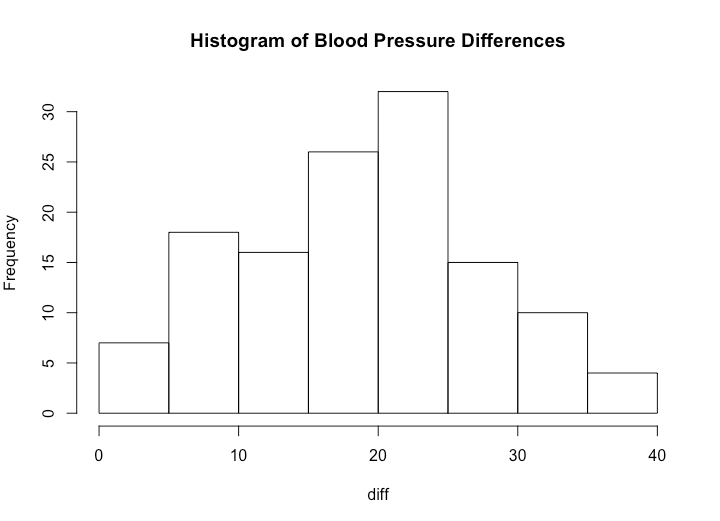
\includegraphics[scale=0.4]{images/diffhist.png}
    \end{center}
\end{frame}

\begin{frame}{Inference for Paired Data}
    Consider some sample statistics for these differences:
    \begin{table}[]
        \centering
        \begin{tabular}{ccc}
            \hline
            $n_{\text{diff}}$ & $\bar{x}_{\text{diff}}$ & $s_{\text{diff}}$ \\
            128 & 18.83 & 8.45 \\
            \hline
        \end{tabular}
    \end{table}
    Taking the differences is going to make our lives easy!
\end{frame}

\begin{frame}{Example}
    Let's run the hypothesis test for our researcher looking at blood pressure medication. We'll test at the $\alpha=0.01$ level.
    
    \begin{table}[]
        \centering
        \begin{tabular}{ccc}
            \hline
            $n$ & $\bar{x}_{\text{diff}}$ & $s_{\text{diff}}$ \\
            128 & 18.83 & 8.45 \\
            \hline
        \end{tabular}
    \end{table}
\end{frame}

\begin{frame}{Example: Climate}
    We have a set of temperatures taken at 197 locations in 1948 and in 2018. We want to know if there were more days exceeding 90$^o$ in 2018 or in 1948. 
    
    \vspace{12pt}
    Is there a relationship between the observations in 1948 and 2018? Or are they independent?
\end{frame}

\begin{frame}{Example: Climate}
    The difference in number of days exceeding 90$^o$ was calculated for each location (days in 2018 - days in 1948). The sample statistics for these differences are:
    \begin{table}[]
        \centering
        \begin{tabular}{ccc}
            \hline
            $n$ & $\bar{x}_{\text{diff}}$ & $s_{\text{diff}}$ \\
            197 & 2.9 & 17.2 \\
            \hline
        \end{tabular}
    \end{table}
    
    Test whether there were more days exceeding 90$^o$ in 2018 or in 1948.
\end{frame}
